%%% LaTeX Template: Two column article
%%%
%%% Source: http://www.howtotex.com/
%%% Feel free to distribute this template, but please keep to referal to http://www.howtotex.com/ here.
%%% Date: February 2011

%%% Preamble
\documentclass[	DIV=calc,%
							paper=a4,%
							fontsize=12pt,%
							onecolumn]{scrartcl}	 					% KOMA-article class

\usepackage{lipsum}													% Package to create dummy text
\usepackage[brazil]{babel}										% English language/hyphenation
\usepackage[protrusion=true,expansion=true]{microtype}				% Better typography
\usepackage{amsmath,amsfonts,amsthm}					% Math packages
\usepackage[pdftex]{graphicx}									% Enable pdflatex
\usepackage[svgnames]{xcolor}									% Enabling colors by their 'svgnames'
\usepackage[hang, small,labelfont=bf,up,textfont=it,up]{caption}	% Custom captions under/above floats
\usepackage{epstopdf}												% Converts .eps to .pdf
\usepackage{subfig}													% Subfigures
\usepackage{booktabs}												% Nicer tables
\usepackage{fix-cm}													% Custom fontsizes
\usepackage[utf8]{inputenc}
\usepackage[top=2.5cm, bottom=2.5cm, left=2.5cm, right=2.5cm]{geometry}
\usepackage[ddmmyyyy]{datetime}
\addto\captionsenglish{%
	\renewcommand\tablename{Tabela}
	\renewcommand\figurename{Figura}
} 
 

 
%%% Custom sectioning (sectsty package)
\usepackage{sectsty}													% Custom sectioning (see below)
\allsectionsfont{%															% Change font of al section commands
	\usefont{OT1}{phv}{b}{n}%										% bch-b-n: CharterBT-Bold font
	}

\sectionfont{%																% Change font of \section command
	\usefont{OT1}{phv}{b}{n}%										% bch-b-n: CharterBT-Bold font
	}



%%% Headers and footers
\usepackage{fancyhdr}												% Needed to define custom headers/footers
	\pagestyle{fancy}														% Enabling the custom headers/footers
\usepackage{lastpage}	

% Header (empty)
\lhead{}
\chead{}
\rhead{}
% Footer (you may change this to your own needs)

%% ====================================
%% ====================================
%% mude o rodape  do projeto
%% ====================================
%% ====================================

\lfoot{\footnotesize \texttt{Cabeamento estruturado} \textbullet ~ Projeto de Redes da empresa JSG}


\cfoot{}
\rfoot{\footnotesize página \thepage\ de \pageref{LastPage}}	% "Page 1 of 2"
\renewcommand{\headrulewidth}{0.0pt}
\renewcommand{\footrulewidth}{0.4pt}



%%% Creating an initial of the very first character of the content
\usepackage{lettrine}
\newcommand{\initial}[1]{%
     \lettrine[lines=3,lhang=0.3,nindent=0em]{
     				\color{DarkGoldenrod}
     				{\textsf{#1}}}{}}



%%% Title, author and date metadata
\usepackage{titling}															% For custom titles

\newcommand{\HorRule}{\color{DarkGoldenrod}%			% Creating a horizontal rule
									  	\rule{\linewidth}{1pt}%
										}

\pretitle{\vspace{-30pt} \begin{flushleft} \HorRule 
				\fontsize{50}{50} \usefont{OT1}{phv}{b}{n} \color{DarkRed} \selectfont 
				}

%% ====================================
%% ====================================
%% mude o titulo  do projeto
%% ====================================
%% ====================================

\title{ Projeto de Redes da empresa JSG}					% Title of your article goes here

%% ====================================



\posttitle{\par\end{flushleft}\vskip 0.5em}

\preauthor{\begin{flushleft}
					\large \lineskip 0.5em \usefont{OT1}{phv}{b}{sl} \color{DarkRed}}
\author{Heltton Mendonça Mendes Maciel }  	% Author name goes here


\postauthor{\footnotesize \usefont{OT1}{phv}{m}{sl} \color{Black} 
					\\Transportadora JSG - Departamento de Tecnologia da informação								% Institution of author
					\par\end{flushleft}\HorRule}

\date{}																				% No date




%%% Begin document
\begin{document}
\maketitle
\thispagestyle{fancy} 	
\thispagestyle{empty}		% Enabling the custom headers/footers for the first page 
% The first character should be within \initial{}




%% ====================================
%% ====================================
%% mude o resumo  do projeto
%% ====================================
%% ====================================
\initial{E}\textbf{este documento detalha o projeto de  implantação de uma nova estrutura de redes da transportadora JSG, empresa que possui duas unidades na cidade de Curitiba. 
Esse projeto prevê a interligação logica entre as unidades, a construção da estrutura fisica necessária, equipamentos a ser utilizado, definição das tecnologias, marcas, tipo de cabeamento e documentação da rede. }

%% ====================================
\begin{figure}
	\centering
	
\includegraphics{utfpr}
\end{figure}

\vspace{3cm}
\centerline{\textit{\textbf{\today}}}

\clearpage
    \renewcommand*\listfigurename{Lista de figuras}
\listoffigures

\renewcommand*\listtablename{Lista de tabelas}
\listoftables




\clearpage
\renewcommand{\contentsname}{Sumário}
\tableofcontents
\clearpage

%% ====================================
%% ====================================
%% Inicio do texto
%% ====================================
%% ====================================
\section{Introdução}
	A transportadora JSG é uma empresa de grande porte com duas unidades na cidade de Curitiba, é responsável pelo transporte dos caminhões que saem da fábrica da Volvo, tratores e colheitadeiras da fábrica da CNH, transporte dos carros da Renault, Nissan e Audi além de atender a demanda de transporte de peças e demais equipamentos das fabricas mencionadas. 
	A empresa atualmente conta com 800 funcionários e aproximadamente 600 desktops/notebooks, 100 coletores de dados, 30 impressoras, aproximadamente 20 equipamentos de rede entre switchs(não gerenciáveis) e hubs e um data center com aproximadamente 8 servidores.
	Esse projeto de redes tem como intuito resolver o problema de quedas, lentidão e segurança relatada pelo cliente, para isso faremos uma nova rede não aproveitando nada da estrutura anterior, será feito a instalação de todos os cabos, ligação entre os switchs, antenas wireless, instalação de equipamentos gerenciáveis, padronizar os ativos de rede com a marca CISCO, criar toda a infraestrutura física e lógica, realizar a “ligação” logica entre as duas unidades da empresa através da tecnologia CISCO ASA.

\subsection{Benefícios}
Após a implantação da nova rede a transportadora JSG terá uma melhor estabilidade na rede da empresa, cabeamento estruturado, documentação da rede, maior segurança tanto logica quanto física, disponibilidade, rede preparada para futura expansão caso necessário, fácil gerenciamento por parte do time de T.I.

\subsection{Organizações Envolvidas}
Coloque o nome de todas as organizações envolvidas. Se for um projeto real, identifique quais as responsabilidades de cada uma das organizações. É comum que em um projeto de redes (cabeamento), temos várias organizações, sendo que cada uma delas com uma determinada responsabilidade.

Sugestão: crie uma tabela contento a relação delas.


\begin{tabular}{|l|l|}
\hline
{\color[HTML]{000000} Responsável}      & {\color[HTML]{000000} Atividade}                                                                                                                                                                                                                                                              \\ \hline
{\color[HTML]{000000} Facilites JSG}    & {\color[HTML]{000000} \begin{tabular}[c]{@{}l@{}}Infraestrutura física para passagem dos cabos,\\ fixação de racks, canaletas, \\ eletrocalhas e toda a parte física na construção\\ da infra necessária.\end{tabular}}                                                                       \\ \hline
{\color[HTML]{000000} Empresa Newtec}   & {\color[HTML]{000000} \begin{tabular}[c]{@{}l@{}}Passagem dos cabos UTP e fibra óptica, fusão \\ de fibra, instalação DIO’S(Distribuidor\\ interno óptico) crimpar cabos, instalação dos \\ patch panel, voice panel, patch\\ cord, instalação física dos switchs e roteadores.\end{tabular}} \\ \hline
{\color[HTML]{000000} Empresa Datatecn} & {\color[HTML]{000000} Certificação do cabeamento de rede}                                                                                                                                                                                                                                     \\ \hline
{\color[HTML]{000000} Setor de T.I}     & {\color[HTML]{000000} \begin{tabular}[c]{@{}l@{}}Responsável pelo acompanhamento de toda parte \\ física e de total responsabilidade da\\ configuração lógica.\end{tabular}}                                                                                                                  \\ \hline
\end{tabular}

\section{Estado atual}
	Atualmente a rede da transportadora JSG não possui nenhum tipo de cabeamento estruturado, documentação, padronização de equipamentos e composta em sua grande maioria de Hubs “cascateado”.  
	Cabeamento antigos e danificados, tecnologia obsoleta, dessa forma não ser aproveitado os passivos de rede que se encontram na empresa.
	O principal motivo que a empresa resolveu reestruturar sua empresa é devido à enorme quantidade de falhas, indisponibilidades, lentidão, segurança da rede, precária comunicação com a outra unidade.

\section{Requisitos}


\begin{tabular}{l}
{\color[HTML]{000000} 1 Nova infraestrutura}                              \\
{\color[HTML]{000000} 2 Novo Cabeamento}                                  \\
{\color[HTML]{000000} 3 Novos equipamentos padronizados CISCO}            \\
{\color[HTML]{000000} 4 Treinamento do time de T.I nas novas tecnologias} \\
{\color[HTML]{000000} 5 Novos links de Internet}                         
\end{tabular}


\section{Usuários e Aplicativos}

Os usuários utilizam em sua grande maioria um ERP para controlar a entrada e saída das cargas, atualmente são aproximadamente 600 usuários, com um controlador de domínio AD(Active Directory). A empresa estima a criação de mais duas unidades, uma na região do ABC em São Paulo para atender montadoras de lá e outra em Sapucaia no Rio Grande do Sul, uma estimativa de mais 600 usuários e pontos de rede.
 

\subsection{Usuários}

\begin{tabular}{|l|l|c|l|}
\hline
{\color[HTML]{000000} \textbf{\begin{tabular}[c]{@{}l@{}}Tipo\\ de Usuário\end{tabular}}} & \textbf{Setor}                                                                   & \multicolumn{1}{l|}{\textbf{Quantidade}} & \textbf{Observação}                                                                                                                                                 \\ \hline
{\color[HTML]{000000} Administrador}                                                      & \begin{tabular}[c]{@{}l@{}}Tecnologia\\ da \\ Informação\end{tabular}            & 12                                       & \begin{tabular}[c]{@{}l@{}}Os usuários\\ de T.I são administradores locais\\ e de domínio, utilizando para \\ manutenção e continuação do \\ ambiente.\end{tabular} \\ \hline
{\color[HTML]{000000} \begin{tabular}[c]{@{}l@{}}Key\\ User\end{tabular}}                 & \begin{tabular}[c]{@{}l@{}}Setores\\ Diversos\end{tabular}                       & 10                                       & \begin{tabular}[c]{@{}l@{}}São usuários da diretoria e gerencia\\ que possui acesso a todos os \\ sistemas da empresa.\end{tabular}                                 \\ \hline
{\color[HTML]{000000} Administrativos}                                                    & \begin{tabular}[c]{@{}l@{}}Comercial/\\ Financeiro/\\ RH/\\ Compras\end{tabular} & 80                                       & \begin{tabular}[c]{@{}l@{}}Funcionários com acesso a ERP \\ especifico correspondente ao seu\\ setor e com acesso à internet\\ liberado.\end{tabular}               \\ \hline
{\color[HTML]{000000} Default}                                                            & \begin{tabular}[c]{@{}l@{}}Demais\\ setores\end{tabular}                         & 488                                      & \begin{tabular}[c]{@{}l@{}}Usuários que utilizam os ERP\\ da empresa com acesso exclusivo as \\ áreas que demandam sua função.\end{tabular}                         \\ \hline
\end{tabular}

\subsection{Aplicativos}

\begin{tabular}{|l|c|l|}
\hline
{\color[HTML]{000000} \textbf{Aplicativo}}                                              & \multicolumn{1}{l|}{\textbf{Setor}} & \textbf{Observação}                                                                                                                                      \\ \hline
{\color[HTML]{000000} \begin{tabular}[c]{@{}l@{}}Software\\ Green Road\end{tabular}}    & Alta                                & \begin{tabular}[c]{@{}l@{}}Software utilizado para\\ monitoramento dos caminhões,\\ é o principal software da empresa.\end{tabular}                      \\ \hline
{\color[HTML]{000000} ERP JSG CORP}                                                     & Alta                                & \begin{tabular}[c]{@{}l@{}}Software responsável pelo \\ controle de entrada e saída das\\ cargas, geração de NF e\\ documentação de viagem.\end{tabular} \\ \hline
{\color[HTML]{000000} \begin{tabular}[c]{@{}l@{}}ERP JSG\\ Administrativo\end{tabular}} & Alta                                & \begin{tabular}[c]{@{}l@{}}Software utilizado pelas áreas \\ administrativas, comercial e compras.\end{tabular}                                          \\ \hline
{\color[HTML]{000000} ERP SKP}                                                          & Alta                                & \begin{tabular}[c]{@{}l@{}}Software utilizado para acompanhamento \\ das manutenções dos veículos.\end{tabular}                                          \\ \hline
\end{tabular}


\section{Estrutura predial existente}

Explique aqui a planta física dos prédios
Pode ser anexada, em escala ou não.

Deve conter uma descrição geral, indicando a possível distância entre os pontos de rede e restrições de instalação.

\section{Planta Lógica - Elementos estruturados}

\subsection{Estado atual}
Deve ter a planta atual, se for o caso

\subsection{Topologia}
Proposta futura, proposta após implantação.
Deve conter o diagrama da rede. Atente-se a redundância  e ligações truncadas.
Deve explicar todos termos e componentes utilizados nestas plantas. Por exemplo: entrance facility, work area, horizontal cabling, etc..

Todos os elementos das figuras devem ser explicados. 
Crie esboço da configuração dos racks e brackets. Explique cada um dos componentes. Você pode criar uma 
 contendo figuras dentro, ou criar uma tabela e incluí-la como imagem. Por exemplo, verifique a tabela \ref{tab1}.

\begin{table}[h!]
\centering
\caption{Exemplo de tabela explicativa}
\label{tab1}
\begin{tabular}{|l|l|l|}
\hline
\multicolumn{3}{|l|}{Figura na Tabela} \\ \hline
1        & Rack          & 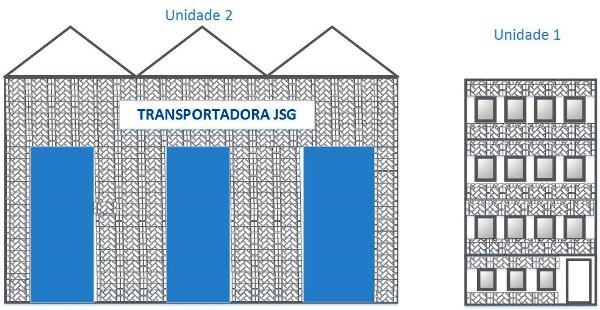
\includegraphics[scale=0.2]{fig1}        \\ \hline
2        & Rack 2        & 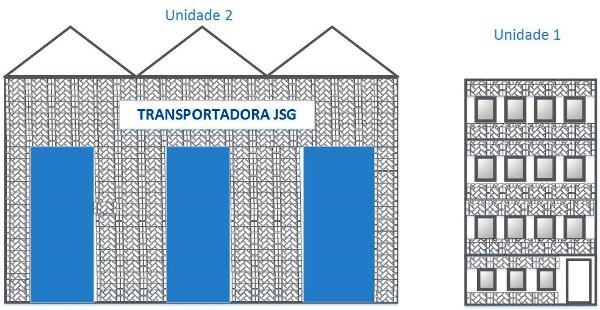
\includegraphics[scale=0.2]{fig1}        \\ \hline
\end{tabular}
\end{table}

\subsection{Encaminhamento}
Eletrodutos, calhas, e qualquer material em que os cabos serão alojados/alocados.

\subsection{Memorial descritivo}

Relacione todos os equipamentos passivos que serão utilizados, tipo, fabricante, quantidade.

\subsection{Identificação dos cabos}
Explique como os cabos serão identificados em seu projeto. Coloque uma relação dos cabos instalados e identificados.

\section{Implantação}
Estabeleça um cronograma de implantação:
Remoção de equipamentos existentes (destino para descarte), instalação dos condutores, instalação dos cabos, 
identificação dos cabos, montagem dos racks, certificação, etc... Crie atividades e estabeleça o tempo de execução. Se for um projeto real, indique também quais os responsáveis pela execução do projeto e de cada uma das etapas.

Defina marcas (e padrões) e fornecedores se for o caso. Atenção a contratados e subcontratados para a realização das atividades. Estabeleça a responsabilidade de execução da atividade e também da validação dela.

Utilize algum software para gerear o cronograma. Excel,etc. O fundamental é dividir em etapas, descrever e estimar o tempo de cada uma delas.

Segue uma relação de ferramentas:
http://asana.com/, 
https://trello.com/, 
http://www.ganttproject.biz/, 
http://www.orangescrum.org/. 

\section{Plano de certificação}
Quais seriam as etapas para a certificação? 
Quais os locais e horários para execução da certificação na rede? Toda rede será certificada?
Como os testes seriam executados?
Quais relatórios de certificação serão (ou deveriam ser) entregues? 

\section{Plano de manutenção}

Revisões periódicas na rede, emissão de certificados para novos pontos.

\subsection{Plano de expansão}
Existe um plano de expansão? Quantos novos pontos poderão ser acrecidos na rede, antes de migração de equipamentos na camada 2? Se houver expansão, quais equipamentos deverão ser direcionados para as estremidades da rede? 

\section{Risco}
Enumerar e explicar os riscos do projeto.

\section{Orçamento}
Crie uma relação de orçamentos baseado na seções anteriores.

\section{Recomendações}
Observações e recomendações para o cliente.

\section{Referências bibliográficas}
Utilize o mendley, o jabref ou diretamente o bibtex para gerenciar suas referências biliográficas. As referências são criadas automaticamente de acordo com o uso no texto.

Exemplo: Redes de computadores, segundo \cite{t2013} é considerada..... Já \cite{kurose2010} apresenta uma versão...

Analisando os pressupostos de \cite{ref3} e \cite{ref4} concluimos que....


\renewcommand\refname{} %%Referências bibliográficas}  
\bibliographystyle{ieeetr}
\bibliography{referencias}  

%% ***********************************************************************
%% === remover daqui =====================================================
%% ***********************************************************************
=================================================
\section{Elementos textuais - Alguns exemplos}

Esta seção apresenta exemplos de elementos textuais. \textbf{Remova-a da versão final do texto}.


\subsection{Colocar elementos em itens}

Texto antes da lista

\begin{itemize}
	\item First item in a list 
	\item Second item in a list 
	\item Third item in a list
\end{itemize}

\subsubsection{Uma subseção de terceiro nivel}

Exemplo de uma subseção

\subsection{Tabelas}

Utilize o site http://www.tablesgenerator.com/ para elaborar as tabelas de seu trabalho.
Para adicionar uma tabela utilize: a tag input, passando o arquivo da tabela como parametro

\begin{table}[h!] % coloque h! para forcar a posicao
\centering
\caption{Modifique a legenda e crie um label}
\label{tab2} %com este label vc faz referencia no texto
\begin{tabular}{|l|l|l|l|l|}
\hline
\multicolumn{1}{|c|}{\textbf{Este é um exemplo de tabela}} & \multicolumn{2}{c|}{\textbf{C1}} & \multicolumn{2}{c|}{\textbf{C2}} \\ \hline
Você pode criar a tabela no excel                          & 1              & 2               & 3               & 4              \\ \hline
Exportar para CSV                                          & 5              & 6               & 7               & 8              \\ \hline
E importar no Table Generator                              & 9              & 10              &                 &                \\ \hline
\multicolumn{5}{|c|}{\textit{Gere o tex, e adicione em seu arquivo}}                                                             \\ \hline
\end{tabular}
\end{table}

Dentro do arquivo você deve definir o label e pode utilizá-lo para referenciar. Exemplo:
Na tab \ref{tab2} temos a relação de ....


Você também pode modificar a tabela manualmente, incluindo, por exemplo h! dentro de sua definição. Veja no exemplo tab2.tex

\subsection{Figuras}

As figuras podem ser no formato PDF, JPG, PNG. Você pode referenciá-las da mesma maneira que tabelas. Exemplo: A figura \ref{fig1} apresenta.....

Não se preocupe o local em que a figura será renderizada em seu texto. Preocupe-se em criar referência para ela, ou seja, toda figura e tabela deve conter pelo menos uma referência no texto.

\begin{figure}
\centering
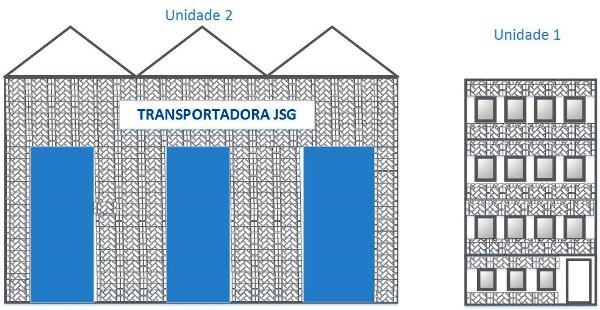
\includegraphics[width=\textwidth]{fig1}
\caption{Exemplo de figura com escala horizontal}
\label{fig1}
\end{figure}


\begin{figure}
	\centering
	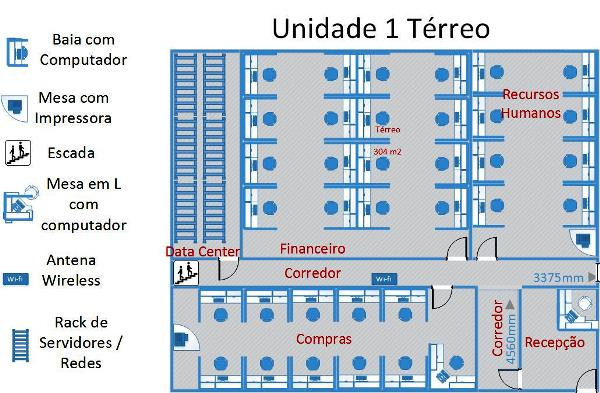
\includegraphics[]{fig2}
	\caption{Exemplo de figura sem escala}
	\label{fig2}
\end{figure}

Você pode rotacionar figuras também. Para isso utilize o parâmetro angle=-90. Repare que a escala da figura foi modificada pelo parametro height. Você também pode utilizar scale

\begin{figure}
	\centering
	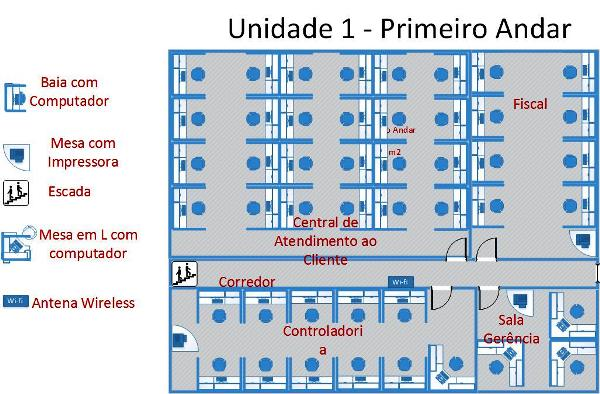
\includegraphics[height=\textwidth,angle=-90]{fig3}
	\caption{Exemplo de figura rotacionada}
	\label{fig3}
\end{figure}


%% ***********************************************************************
%% === ate aqui    =====  ================================================
%% ***********************************************************************

\end{document}